\documentclass[a4paper]{report}

%====================== PACKAGES ======================

\usepackage[svgnames]{xcolor}
\usepackage[french]{babel}
%pour gérer les positionnement d'images
\usepackage{float}
\usepackage{graphicx}
\usepackage[colorinlistoftodos]{todonotes}
\usepackage{url}
%pour les informations sur un document compilé en PDF et les liens externes / internes
\usepackage{hyperref}
%pour la mise en page des tableaux
\usepackage{array}
\usepackage{tabularx}
%pour utiliser \floatbarrier
%\usepackage{placeins}
%\usepackage{floatrow}
%espacement entre les lignes
\usepackage{setspace}
%modifier la mise en page de l'abstract
\usepackage{abstract}
%police et mise en page (marges) du document
\usepackage[T1]{fontenc}
\usepackage[top=2cm, bottom=2cm, left=2cm, right=2cm]{geometry}
%Pour les galerie d'images
\usepackage{subfig}
\usepackage{}
\usepackage{xcolor}
\usepackage{framed}
\usepackage{fontspec}
\usepackage{xunicode}
\usepackage{hyperref}
\usepackage{pifont}
\usepackage{amsthm,thmtools,amssymb, amsmath, mathtools} %pour les mathématiques
\colorlet{shadecolor}{lightgray!25}
\usepackage{algorithm}
\usepackage[end]{algpseudocode}

\usepackage{fancyhdr}
\usepackage{lastpage}

\pagestyle{fancy}
\renewcommand\headrulewidth{1pt}
\fancyhead[L]{Gestion des noeuds isolés en LoRa}
\fancyhead[R]{URCA}
\renewcommand\footrulewidth{1pt}
\fancyfoot[L]{HERARD Joffrey}
\fancyfoot[C]{
\textbf{Page \thepage/\pageref{LastPage}}}
\fancyfoot[R]{2017-2018}
\setlength{\headheight}{14pt}
%====================== INFORMATION ET REGLES ======================
%rajouter les numérotation pour les \paragraphe et \subparagraphe
\setcounter{secnumdepth}{4}
\setcounter{tocdepth}{4}

\hypersetup{							% Information sur le document
pdfauthor = {HERARD JOFFREY}			% Auteurs
pdftitle = {Stage -
			Gestion des noeuds isolés en LoRa},			% Titre du document
pdfsubject = {Rapport de Stage},		% Sujet
pdfkeywords = {Tag1, Tag2, Tag3, ...},	% Mots-clefs
pdfstartview={FitH}}					% ajuste la page à la largueur de l'écran
%pdfcreator = {MikTeX},% Logiciel qui a crée le document
%pdfproducer = {}} % Société avec produit le logiciel

\newcommand{\cmark}{\ding{51}}%
\newcommand{\xmark}{\ding{55}}%

\newtheorem{post}{Postulat}
\newtheorem{mydef}{Définition}
%%
%======================== DEBUT DU DOCUMENT ========================

\usepackage{minted}
\begin{document}

%régler l'espacement entre les lignes
\newcommand{\HRule}{\rule{\linewidth}{0.5mm}}

%page de garde
\begin{titlepage}
\begin{center}

% Upper part of the page. The '~' is needed because only works if a paragraph has started.

\includegraphics[width=0.35\textwidth]{./logo}~\\[1cm]

\textsc{\LARGE UFR Sciences Exactes et Naturelles}\\[1.5cm]

\textsc{\Large }\\[0.5cm]

% Title
\HRule \\[0.4cm]

{\huge \bfseries  
Gestion des noeuds isolés en LoRa\\[0.4cm] }

\HRule \\[1.5cm]

% Author and supervisor
\begin{minipage}{0.4\textwidth}
\begin{flushleft} \large
\emph{Auteur:}\\
HERARD \textsc{Joffrey}\\
%\emph{Collaborateur:}\\
%POUEY \textsc{Patrick}\\
\end{flushleft}
\end{minipage}
\begin{minipage}{0.4\textwidth}
\begin{flushright} \large
\emph{Responsables:} \\
Olivier \textsc{FLAUZAC}\\
Florent \textsc{NOLOT}\\
Philipe \textsc{COLA}\\
\end{flushright}
\end{minipage}

\vfill

% Bottom of the page
{\large 2017-2018}

\end{center}
\end{titlepage}
% ok correction ? 

%page blanche
\newpage
~
%ne pas numéroter cette page
\thispagestyle{empty}
\newpage

\renewcommand{\abstractnamefont}{\normalfont\Large\bfseries}
%\renewcommand{\abstracttextfont}{\normalfont\Huge}

\begin{abstract}
\hskip7mm

\begin{spacing}{1.3}
La problémablique de notre étude portant sur la gestion des noeuds isolés en \textit{LoRa}. Nous expliquerons les problèmes que peut présenter une architecture \textit{LoRaWAN} et proposerons diverses solutions pour les résoudre. Avant de procéder à l'implémentation des ces diverses solutions nous exécuterons des simulations sur le modèle de communication \textit{LoRa} avec les algorithmes présentés auparavant. Par la suite, il a été expliquer comment programmer cette solution dans un capteur via l'utilisation de capteurs \textit{LoPy} voir même \textit{Discovery} basé sur les puces ST32. \end{spacing}
\end{abstract}
% ok correction ? 

\tableofcontents
\thispagestyle{empty}
\setcounter{page}{0}
%ne pas numéroter le sommaire

\newpage

%espacement entre les lignes d'un tableau
\renewcommand{\arraystretch}{1.5}

%====================== INCLUSION DES PARTIES ======================

\thispagestyle{empty}
%recommencer la numérotation des pages à "1"
\setcounter{page}{0}
\newpage

	   
\chapter{Présentation du sujet}
 
\section{Sujet}
 Tout d'abord pour comprendre l'étendu du sujet il est nécéssaire de bien comprendre tout d'abord l'ensemble des termes qui le décrivent. 

\begin{mydef}
 Noeuds isolés : En effet, le  \textit{LoRaWAN} est basé sur un modèle d'infrastructure. Par exemple, quand est-il d'un noeud qui n'est pas visible par une  \textit{LoRaWAN} Gateway? Il y a deux cas de figures simple : le premier cas est celui  ou le noeud n'est visible d'aucun device et d'aucune gateway  \textit{LoRaWAN}. Dans ce cas il n'y a rien à faire le noeud est isolé de manière permanente. Le deuxième cas de figure est celui qui nous intéresse particulièrement ici, en effet le noeud isolé est visible par un end-device qui lui est à porté d'une  \textit{LoRaWAN} Gateway tout comme l'illustre le schéma suivant :
 \begin{figure}[h!]
\centering
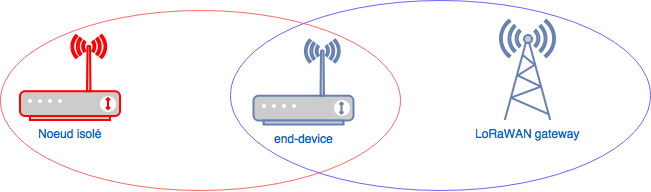
\includegraphics[scale=0.6]{probleme.png} 
\caption{Problème des noeuds isolés}
\end{figure}
\end{mydef}
 

Les objectifs sont donc de gérer les noeuds isolés. Le tout en étant capable de faire et de respecter un ensemble de choses : 
\begin{enumerate}
	\item Récupérer les informations détenue par les capteurs/noeuds isolé.
	\item Gérer les noeuds isolés de sortes a ne pas leur faire gaspiller de l'energie trop souvent.
	\item Faire en sorte que du point de vue du serveur réseaux et de SPOT les noeuds isolés soit actif.
	\item Développer des classes/libraires pour utiliser l'algorithme de manière transparente.
\end{enumerate}

Le prochain chapitre décrit le fonctionnement ainsi que l'architecture d'un Réseaux LoRaWAN dit classique. C'est à dire le réseaux avant l'implémentation d'un algorithme comme celui présenté au travers de ce rapport.
\chapter{LoRaWAN}
Comment connecter les milliards de capteurs qui seront potentiellement déployés dans le monde et qui participeront à la construction des villes intelligentes, de la mobilité et de l'industrie du futur ? \newline
Il existe bon nombre de réponses à cette question mais nous pourrons en trouver assurément du côté des LPWAN. Par conséquent nous commenceront par développer ce modèle avant de décrire la spécification de version 1.0 de  \textit{LoRaWAN}, basé sur \textit{LoRa}.
\subsection{Convention de nommage }
Afin de conserver une certaine cohérence vis à vis de la spécification des termes anglo-saxons, nous avons préféré les conserver dans ce document. Toute fois, vous en trouverez une brève définition ci-dessous : 
\begin{itemize}
\item End-devices : Définissent les périphériques cibles comme les capteurs par exemple.
\item Isolated-devices/Isolated Nodes : Définissent les périphériques cibles comme les capteurs par exemple  mais cette fois ci. Isolé par rapport à une gateway  \textit{LoRaWAN}.
\item Uplink : Correspond aux chemins réseaux des end-devices vers le serveur réseaux. 
\item Downlink : Correspond aux chemins réseaux du serveur vers le end-devices. 
\item Gateway : Correspond aux concentrateurs réseaux. 
\item LoRaGateway : Correspond aux concentrateurs réseaux qui sont des end-devices . 
\end{itemize}



\subsection{LPWAN}
Pour certaines applications (villes intelligentes, maintenance prédictive, agriculture connectée, etc.), il s'agit de déployer des centaines de milliers de capteurs (monitoring énergétique, qualité de l'air, gestion des déchets) fonctionnant sur pile et communiquant quotidiennement de très faibles quantités de données, à faible débit vers des serveurs sur Internet (cloud).Les réseaux LPWAN, comme le laisse deviner l'acronyme, sont des réseaux sans fil basse consommation, bas débit et longue portée, optimisés pour les équipements aux ressources limitées pour lesquels une autonomie de plusieurs années est requise. Ces réseaux conviennent particulièrement aux applications qui n'exigent pas un débit élevé.
Contrairement aux opérateurs mobiles les LPWAN utilisent des bandes de fréquences à usage libre, disponibles mondialement et sans licence : ISM (Industriel, Scientifique et Médical). Compte tenu des faibles débits et de la faible occupation spectrale des signaux, il faut en moyenne, pour un réseau LPWAN, 10 fois moins d'antennes pour couvrir la même surface qu'un réseau cellulaire traditionnel.
\subsection{LoRaWAN}
\textit{LoRaWAN} (Long Range Radio Wide Area Network) est un réseau LPWAN basé sur la technologie radio \textit{LoRa}.
Cette technologie, développée par Cycleo en 2009 puis rachetée, 3 ans après, par l'américain Semtech, utilise une technique d'étalement de spectre pour la transmission des signaux radio (chirp spread spectrum). 
La technologie \textit{LoRa}, à travers le réseau  \textit{LoRaWAN}, est poussée par un consortium d'industriels et d'opérateurs nommé \textit{LoRa} Alliance qui regroupe notamment IBM, Cisco, Bouygues Télécom, etc…
\subsubsection{LoRa Alliance}
La \textit{LoRa} Alliance est une association dont le but, non lucratif, est de standardiser le réseau  \textit{LoRaWAN} pour apporter à l'internet des objets (IoT) un moyen fiable pour se connecter à Internet. Cette association a été créée par Semtech et de nombreux acteurs industriels garantissent aujourd'hui l'interopérabilité et la standardisation de la technologie \textit{LoRa}. 







\subsubsection{Les différentes couches d'un réseaux LoRaWAN}
\begin{figure}[h!]
\centering
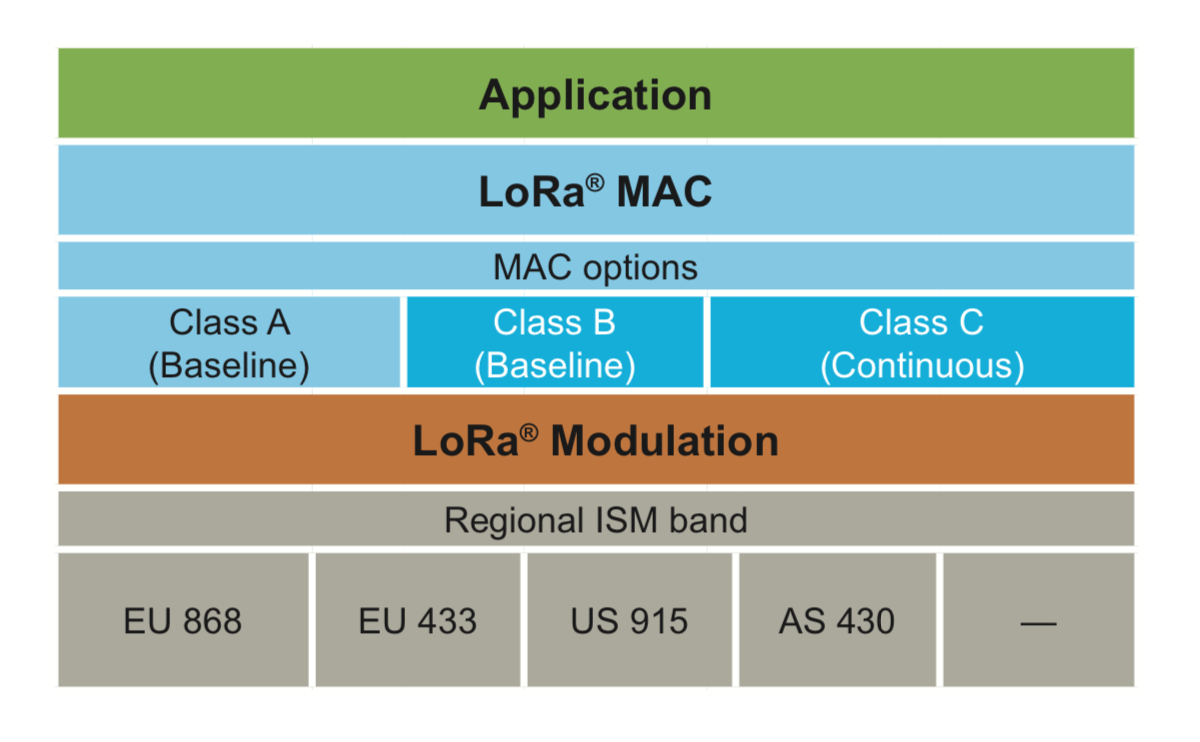
\includegraphics[scale=0.6]{couchelora.png}
\caption{Les différentes couches d'un réseau LoRaWAN}
\end{figure}
On peut alors constater que la couche physique fournie par la technologie \textit{LoRa} n'est pas suffisante pour assurer la communication réseau. En définissant le protocole réseau (\textit{LoRa} MAC), pour une communication d'équipements \textit{LoRa} à travers un réseau, le protocole  \textit{LoRaWAN} assure une communication bi-directionnelle et définit trois classes d'équipements différents. Nous définirons celles-ci dans la partie de notre étude consacrée à l'explication des différences sur les messages, les fenêtres de réception...
\newpage
\subsubsection{Différence entre le LoRa et LoRaWAN}
D'un côté,  \textit{LoRaWAN} est un modèle d'architecture réseaux qui exploite la technologie radio \textit{LoRa} pour faire communiquer les gateways avec les périphériques et les capteurs. En outre, nous détaillerons les particularités de cette architecture réseaux dans le point suivant. A noter, au sein de notre document, la présence de raccourcis d'écriture désignant \textit{LoRa} comme la communication spécifiée en réseau  \textit{LoRaWAN} mais il s'agira bel et bien d'échanges effectués en \textit{LoRa} avec une couche \textit{LoRa} MAC. 
 
\subsubsection{Architecture d'un réseaux LoRaWAN}
\begin{figure}[h!]
\centering
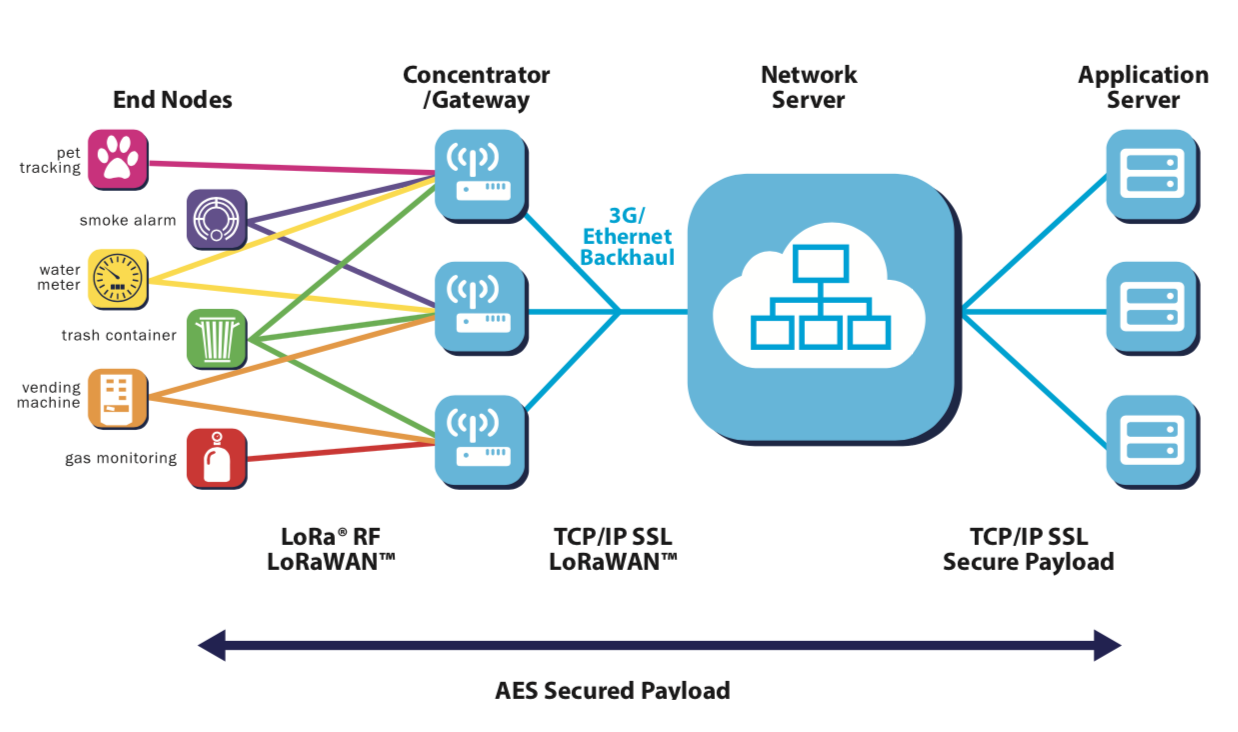
\includegraphics[scale=0.6]{networkArch.png}
\caption{Architecture d'un réseaux LoRaWAN}
\end{figure}
Cette figure représente une architecture classique d'un réseau  \textit{LoRaWAN}. Typiquement un réseau  \textit{LoRaWAN} est en topologie "star of star" étoile en étoile, le centre de cette topologie est le serveur de réseau qui assure la gestion du débit adaptatif, de la sécurité des données ou encore de la redondance des données. Celui ci est entouré d'un côté par les gateways connectés en ethernet/4G au serveur de réseau, auquel les end-devices seront connectés, eux en \textit{LoRa}. D'autre part du serveur réseaux, nous avons les serveur d'applications lié par ethernet, ces mêmes serveur d'application lié elle mêmes à une interface web ( échange HTTP, MQTT).
Une des particularités d’un réseau  \textit{LoRaWAN}, est qu’un équipement ne communique pas exclusivement à travers un concentrateur. Tous les concentrateurs couvrant l’équipement peuvent recevoir les données transmises par ce dernier.
Cela facilite grandement la communication avec les équipements en mobilité en dispensant le réseau de mécanismes de hand-over (passage d’un concentrateur à un autre) qui auraient pour effet de complexifier sa gestion et très probablement de réduire ses performances. Par contre, lorsque le serveur envoie un message à destination d’un équipement, c’est par le biais d’un seul concentrateur. C’est le cas en particulier des messages requérant un acquittement par le serveur.
 assure l'échange entre le serveur de réseaux et les serveurs d'applications : AppsKey. La sécurité après ces serveurs n'est plus géré par la spécification  \textit{LoRaWAN}.
 

\subsubsection{Sécurité d'un réseaux LoRaWAN}
Une question importante est aussi celle de la sécurité a travers le réseaux, on parle de capteurs voir d'un ensemble d'informations qui vont communiqué, donc c'est une question importante, et surtout ça concerne l'Internet des Objets dans son ensemble .
La sécurité est assuré de bout en bout par un chiffrement AES-128 bits, elles sont aux nombre de deux, la première qui couvre les capteurs jusqu'au serveur réseaux nommé NwkSKey.
\begin{itemize}
\item Network Session Key (NwkSKey), assure l’authenticité des équipements sur le réseau .
\item Application Session Key (AppSKey), la sécurité et la confidentialité des données transmises à travers le réseau.
\end{itemize}

En d’autre termes, la clé réseau permet à l’opérateur de sécuriser son réseau alors que la clé applicative permet au fournisseur de l’application de sécuriser les données qui transitent à travers le réseau.

Les données utiles que souhaite transmettre sont tout d’abord chiffrées via la AppSKey. Un en-tête, contenant entre autres l’adresse de l’équipement, est ensuite ajouté aux données chiffrées. À partir de cela, le MIC – Message Integrity Code – est calculé via NwkSKey. Le MIC permet au réseau de vérifier l’intégrité des données et de l’équipement sur le réseau. Enfin, le MIC est ajouté au message contenant l’en-tête et les données chiffrées avant transmission.

À réception du message par le serveur de gestion du réseau, ce dernier pourra vérifier l’intégrité des données grâce au MIC tout en préservant la confidentialité des données (chiffrées par AppSKey).
L'ensemble des trames d'échange vont être décrit dans la suite du document.


 % ok correction ? 
\chapter{Solutions}
Il y a  plusieurs pistes de solutions afin de résoudre ce problème. Un end node visible par un noeud isolé peut etre redefinie comme une passerelle $\rightarrow$ On définit donc une \textit{LoRa} Gateway (noté LGW à travers le document)
Il y a donc une redéfinition des acteurs :
\begin{itemize}
\item LoRaWAN Gateway (LWGW)
\item LoRa Gateway 
\item Isolated Node (IN)
\end{itemize}

On aurais la possibilité d'avoir deux modes : 
\begin{itemize}
\item Mode proxy : La LoRaGateway fait un relai en aveugle des données des noeuds Isolés .
\item Mode concentrateur : La LoRaGateway collecte les données des Noeuds Isolés.
\end{itemize}
Il ya tout de même quelque problèmes pour le mode Proxy. 
En effet il y a une certaine compléxité de la mise en oeuvre. Que ce soit au niveau de l'écoute et la captures des échanges par des end-nodes mais aussi de la capture par le End Node de message du Noeud isolé, ou encore de la capture par le End Node de message à destination du Noeud isolé. Il y a aussi une certaine compléxité au niveau de la gestion des synchronisation en fonction des classes energetique des objets. En classez C, le problème se revele pendant les phases démission du End-Node. En classe A et B lors dez la gestion multiple des slots de réception par le un End Node. Il y a un derniere aspect qui est pratique, en effet les bibliothèques, on écoute et collecte des message sans en etre le destinataire. Il y aurais deux solutions pour pallier à cela, soit la mise en place d'un mode promiscuité, soit d'un recodage complet de la spécification.


Ici nous allons nous intéréssé surtout à l'ensemble des algorithmes qui décrive le fonctionnement du mode d'échanges classique entre une LGW et un IN, afin des les appliquer en simulation, puis de réaliser la mise en oeuvre/applications de ceux-ci.

\newpage
\section{Algorithme}


L'ensemble des messsages du système sont de la forme :

\begin{center}
\texttt{< message\_type , source , destination , data >}
\end{center}

On distingue donc plusieurs messages dans le système. On considère qu'à chaque message correspond une fonction portant le nom du message, initialisant le type et la source du message, et prenant en paramètre la destination et les données.

\subsection{les messages IN -> LGW}
\begin{itemize}
    \item les messages \texttt{discover}
    \begin{itemize}
      \item message mis en place pour la découverte d'une \texttt{LGW} par un \texttt{IN}
      \item \texttt{destination = udef} : en broadcast
      \item \texttt{data = udef} : aucune info
    \end{itemize}
    \item les messages \texttt{pair}
    \begin{itemize}
      \item message d'apairage d'un IN sur une LGW
      \item \texttt{data = udef} : aucune info
    \end{itemize}
    \item les messages \texttt{data\_response}
    \begin{itemize}
      \item réponse à une demande de données de la part d'une LGW
    \end{itemize}
\end{itemize}

\subsection{les messages LGW -> IN}
Pour l'ensemble des messages LoRa issus de la \texttt{LGW} la partie data est structurée ainsi :

\begin{itemize}
  \item \texttt{answer\_frequency} : fréquence sur laquelle l'\texttt{IN} doit répondre
  \item \texttt{next\_slot} : délai d'ici la prochaine fenêtre d'écoute
  \item \texttt{next\_duration} : temps fixé de la prochaine fenêtre d'écoute
  \item \texttt{next\_frequency} : fréquence de la prochaine fenêtre d'écoute
  \item \texttt{data} : espace de données spécifiques à l'échange
\end{itemize}

Le message devient donc :

\begin{center}
\texttt{< message\_type , source , destination , answer\_frequency , next\_slot , next\_duration , next\_frequency , data>}
\end{center}

Les différents messages \texttt{LGW} $\rightarrow$ \texttt{IN} sont donc :
\begin{itemize}
    \item les messages \texttt{candidate} %\textbf{(ce nom ne me plait pas !!!)}
    \begin{itemize}
      \item message de réponse d'une \texttt{LGW} après réception d'un \texttt{discover} d'un \texttt{IN}
      \item \texttt{data = udef} : aucune info
    \end{itemize}
    \item les messages \texttt{data\_request}
    \begin{itemize}
      \item message de demande de données
      \item \texttt{data = udef} si une seule donnée disponible ou \texttt{data = requested\_data} dans le cas de donnés multiples
    \end{itemize}
\end{itemize}

\section{Liste des fonctions utilisées}

\subsection{Fonction d'émission}

\texttt{void sendLora(frequency , message)}

\subsection{Fonction de réception}

la fonction \texttt{listen} écoute sur la fréquence \texttt{frequency} un temps définit par \texttt{time}. Le prototype de cette fonction est :

\begin{center}
\texttt{(message,time) listen(frequency , source , message\_type , time\_listen)}
\end{center}

les valeurs des paramètres de cette fonction sont :
\begin{itemize}
  \item \texttt{frequency} : fréquence d'écoute
  \item \texttt{source} : id de l'émetteur du message
  \begin{itemize}
    \item \texttt{source = udef} : écoute de tous les n{\oe}uds sur la fréquence définie
  \end{itemize}
  \item \texttt{message\_type} : type de message attendu
  \begin{itemize}
    \item \texttt{message\_type = udef} : écoute de tous les types de messages
  \end{itemize}
  \item \texttt{time\_listen} : durée de la fenêtre de réception
  \begin{itemize}
    \item \texttt{time\_listen = udef} : fenêtre infinie
  \end{itemize}
\end{itemize}

Valeurs de retour :

\begin{itemize}
  \item \texttt{message} message reçu
  \begin{itemize}
    \item passage du message dans sa totalité
    \item \texttt{message == udef} : pas de réception respectant les contraintes
  \end{itemize}
  \item \texttt{time} temps restant basé sur \texttt{time\_listen}
  \begin{itemize}
    \item \texttt{time == udef} : dans le cas de \texttt{time\_listen = udef}
  \end{itemize}
\end{itemize}

\section{Algorithme 1 - 1}

\subsection{Algorithme des \texttt{IN}}

\begin{algorithm}
\caption{Initialisation des variables de communication}\label{alg:intvar}
\begin{algorithmic}[1]
\Procedure{$init\_var$}{msg}
\State $lgw \leftarrow msg.source$
\State $freq\_send \rightarrow msg.answer\_frequency$
\State $next\_time \leftarrow msg.next\_slot$
\State $timer \leftarrow msg.next\_duration$
\State $freq\_listen \leftarrow msg.next\_frequency$
\EndProcedure
\State
\Procedure{$flush\_var$}{~}
\State $lgw \leftarrow udef$
\State $msg \leftarrow udef$
\State $next\_time \leftarrow udef$
\State $timer \leftarrow timer\_disco$
\State $freq\_listen \leftarrow freq\_disco$
\State $freq\_send \leftarrow freq\_disco$
\EndProcedure
\end{algorithmic}
\end{algorithm}


\begin{algorithm}
\caption{Algorithme IN 1-1}\label{alg:in1-1}
\begin{algorithmic}[1]
\While{$(true)$}
  \State $flush\_var()$
  \State \Comment{------------------------------------------------------- \textit{phase d'apairage}}
  \While{$(msg = udef)$}
    \State $sendLora(freq\_listen,discover(udef,udef))$
    \State $(msg,t) = listen(freq\_send,udef,candidate,timer + rnd())$
  \EndWhile
  \State $initVar(msg)$
  \State $sendLora(freq\_send,pair(lgw,udef))$
  \State
  \State \Comment{----------------------------------------------\textit{Phase d'échanges}}
  \While{$(lgw != udef)$}
    \State $sleep(next\_time)$
    \State $(msg,t) = listen(freq\_send,lgw,data\_request,timer)$
    \If{$msg != udef$}
      \State $initVar(msg)$
      \State $sendLora(freq\_send,date\_response(lgw,local\_data)$
    \Else
      $flush\_var()$
    \EndIf
  \EndWhile
\EndWhile
\end{algorithmic}
\end{algorithm}

\subsection{Algorithme des \texttt{LGW}}

\begin{algorithm}
\caption{Initialisation des variables de communication}\label{alg:initvarlg}
\begin{algorithmic}[1]
\Procedure{$init\_var$}{~}
\State $freq\_send \rightarrow chose()$
\State $timer \leftarrow chose()$
\State $freq\_listen \leftarrow chose()$
\State $freq\_next \leftarrow chose()$
\EndProcedure
\State
\Procedure{$flush\_var$}{~}
\State $timer \leftarrow timer\_disco$
\State $freq\_listen \leftarrow freq\_disco$
\State $freq\_send \leftarrow freq\_disco$
\State $in \leftarrow udef$
\EndProcedure
\end{algorithmic}
\end{algorithm}

\begin{algorithm}
\caption{Algorithme lgw 1-1}\label{alg:lgw1-1}
\begin{algorithmic}[1]
\State $LoRaWAN\_join()$
\State $flush\_var()$
\While{$(true)$}
  \If{$(in == udef)$}
    \State $(msg,t) = listen(freq\_listen,udef,discover,timer)$
  \EndIf
  \If{$(msg != udef)$}
    \State $in \leftarrow msg.source$
    \State $init\_var()$
    \State $sendLora(freq\_send,candidate(in,freq\_listen,slot,duration,freq\_next,udef)$
    \State $(msg,t) = listen(freq\_listen,in,pair,timer)$
    \If{$(msg == udef)$}
      \State $flush\_var()$
    \EndIf
  \EndIf
  \If{$(in != udef)$}
    \State $init\_var()$
    \State $sendLora(freq\_send,data\_request(in,freq\_listen,slot,duration,freq\_next,udef)$
    \State $(msg,t) = listen(freq\_listen,in,data\_response,timer)$
    \If{$(msg != udef)$}
      \State $send\_lora\_data(id + ":" + local\_data + ";" + in + ":" + msg.data)$
    \Else
      \State $send\_lora\_data(id + ":" + local\_data + ";" + in + ":" + udef)$
      \State $flush\_var()$
    \EndIf
  \EndIf
\EndWhile
\end{algorithmic}
\end{algorithm}

\newpage
\subsection{Algorithme k/1 : k IN <-> 1 LGW}
Ici le seul changement qui opère est celui d'enregistrement de plusieurs noeuds isolés.
\begin{algorithm}
\caption{Algorithme lgw 1-1}\label{alg:lgwk-1}
\begin{algorithmic}[1]
\State $LoRaWAN\_join()$
\State $flush\_var()$
\While{$(true)$}
  \If{$(in == udef)$}
    \State $(msg,t) = listen(freq\_listen,udef,discover,timer)$
  \EndIf
  \If{$(msg != udef)$}
    \State $in \leftarrow msg.source$
    \State $init\_var()$
    \State $sendLora(freq\_send,candidate(in,freq\_listen,slot,duration,freq\_next,udef)$
    \State $(msg,t) = listen(freq\_listen,in,pair,timer)$
    \If{$(msg == udef)$}
      \State $flush\_var()$
    \EndIf
  \EndIf
  \If{$(in != udef )$}
 	 \If{$(in NOT in tabRegisteredIN )$}
 	 	\State $ tabRegisteredIN.append(in)$
 	 \EndIf
  	  \State $init\_var()$
  	  \State $sendLora(freq\_send,data\_request(in,freq\_listen,slot,duration,freq\_next,udef)$
  	 \State $(msg,t) = listen(freq\_listen,in,data\_response,timer)$
   	 \If{$(msg != udef)$}
    	  \State $send\_lora\_data(id + ":" + local\_data + ";" + in + ":" + msg.data)$
    	\Else
    	  \State $send\_lora\_data(id + ":" + local\_data + ";" + in + ":" + udef)$
    	  \State $flush\_var()$
    \EndIf
  \EndIf
\EndWhile
\end{algorithmic}
\end{algorithm}
\newpage
\section{Chronogrammes}
\subsection{Phase de découverte et d'enregistrement}
\begin{figure}[!ht]
\centering
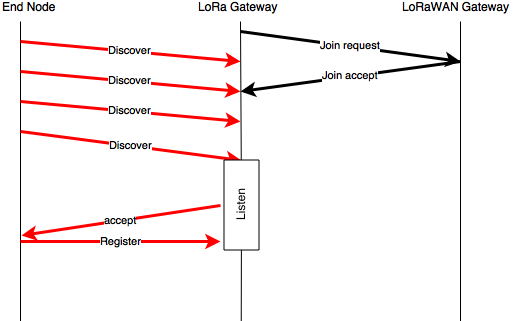
\includegraphics[scale=0.6]{Discovery.png} 
\caption{Phase de découverte}
\end{figure}
\subsubsection{Coté Isolated node}Au début le noeud isolé se reveille, il envoie des messages \textbf{Discover}. Si une \textit{LoRa} Gateway répond par un message \textbf{Accept} le noeud répond alors avec un message  \textbf{Register} pour confirmer son appairage avec la \textit{LoRa} Gateway.
\subsubsection{Coté LoRa Gateway}
La \textit{LoRa} Gateway avant toute opération avec n'importe quel élement de l'environnement doit s'appairer avec une gateway \textit{LoRaWAN} avec la requete  \textbf{Join Request}.
\subsubsection{Coté LoRaWAN Gateway}
La gateway \textit{LoRaWAN} executé un déroulement normal. Elle répond aux requetes join avec un message  \textbf{Join Accept}
\newpage
\subsection{Phase de collecte}
\begin{figure}[!ht]
\centering
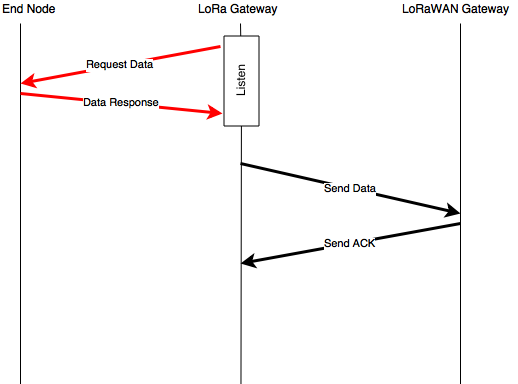
\includegraphics[scale=0.6]{Collect.png} 
\caption{Phase de collecte}
\end{figure}

\subsubsection{Coté Isolated node} Le noeud se reveille à un slot prévu entre la \textit{LoRa} Gateway et le noeud. Tout ceci afin de recevoir la demande de donnée de la part de la gateway \textit{LoRa}. Le noeud répond avec les données dans un message nommé  \textbf{Data Response}.
\subsubsection{Coté LoRa Gateway}
La \textit{LoRa} Gateway va se reveiller pour collecter les données des noeuds qui lui sont accroché. Elle envoit donc un message  \textbf{Request Data} . \\
Mode Concentrateur : Une fois que toutes les données sont reçues, la Gateway assemble les données et envoie à la  \textit{LoRaWAN} gateway. \\
Mode Proxy : Une fois que toutes les données sont reçues, la Gateway usurpe chaque isolated node et envoie les données à la  \textit{LoRaWAN} gateway. Pour finir par envoyé ces propres données.
\subsubsection{Coté LoRaWAN Gateway}
La \textit{LoRaWAN} Gateway accuse la reception des données envoyées par la gateway \textit{LoRa}.
\textbf{Send ACK}
 % ok correction ? 
\newpage
\chapter{Simulation}

\section{Le simulateur : Omnet++}
OMNeT ++ est une bibliothèque et une structure de simulation C ++ extensible, modulaire et basée sur des composants, principalement utilisé pour la construction de simulateurs de réseau. Le terme "réseau" est entendu dans un sens plus large qui inclut les réseaux de communication câblés et sans fil, les réseaux sur puce, les réseaux de mise en file d'attente, et ainsi de suite. Les fonctionnalités spécifiques au domaine telles que la prise en charge de réseaux de capteurs, de réseaux ad-hoc sans fil, de protocoles Internet, de modélisation de performances, de réseaux photoniques, etc., sont fournies par des frameworks de modèles, développés en tant que projets indépendants. OMNeT ++ offre un IDE basé sur Eclipse, un environnement d'exécution graphique et une foule d'autres outils. Il existe des extensions pour la simulation en temps réel, l'émulation de réseau, l'intégration de base de données, l'intégration SystemC et plusieurs autres fonctions.
Même si OMNeT ++ n'est pas un simulateur de réseau en soi, il a acquis une grande popularité en tant que plate-forme de simulation de réseau dans la communauté scientifique ainsi que dans les milieux industriels, et a constitué une importante communauté d'utilisateurs.
Afin de réaliser un ensemble de test/simulation nous avons utilisé Omnet pour ce projet.

Le code des fichiers $C^{++}$ est mis à disposition en Annexes.
\section{Génération des graphes}
Nous avons choisi d'utiliser iGraph, afin de generer des graphes aléatoires.
iGraph est une collection de bibliothèque pour créer et manipuler des graphiques et analyser des réseaux. Il est écrit en C et existe également en tant que paquets Python et R. Il existe de plus une interface pour Mathematica. Le logiciel est largement utilisé dans la recherche universitaire en sciences de réseau et dans des domaines connexes.
iGraph a été développé par Gábor Csárdi et Tamás Nepusz. Le code source des paquets iGraph a été écrit en C. iGraph est disponible gratuitement sous GNU General Public License Version 2.

La génération se fait en plusieurs étapes : 
\begin{enumerate}
\item Récupération des arguments : Nombres de  \textit{LoRaWAN} Gateway, \textit{LoRa} Gateway et de Isolated node.	
\item Création du graphe et ajout du nombre de sommets dont on a besoin.
\item On connecte les  \textit{LoRaWAN} à une  \textit{LoRaWAN} gateway, par définitions ils sont enregistré à au moins une gateway  \textit{LoRaWAN}.
\item On connecte des Isolated Node de manière aléatoire à une LoRa Gateway (au moins une)
\item Ensuite on applique un deuxième tour d'association de noeud à des gateway 	basé sur une méthode  Erdös Renyi : On définit la probabilité d'existence entre deux nœuds, pour chaque couple de nœud, on tire au sort un nombre, si le nombre est inférieur on met le lien.
\item On écrit le fichier .ned qui décrit la configuration du graphe crée. 

\begin{minted}[
frame=lines,
framesep=2mm,
baselinestretch=1.2,
bgcolor=LightGray,
fontsize=\footnotesize,
linenos
]{python}
fic.write("\t\t\t" + ""+nomSommet0+"["+str(num_sommet0)+"].channelsO++" + " --> "
+"{delay="+str(delay1)+"ms;}" + " --> " +
""+nomSommet1+"["+str(num_sommet1)+"].channelsI++" + ";\n")
fic.write("\t\t\t" + ""+nomSommet0+"["+str(num_sommet0)+"].channelsI++" + " <-- "
 +"{delay="+str(delay2)+"ms;}" + " <-- " +
   ""+nomSommet1+"["+str(num_sommet1)+"].channelsO++" + ";\n")
\end{minted}

\end{enumerate}
Par exemple voici le résultat graphique réalisé avec GraphViz :

\begin{figure}[!ht]
\centering
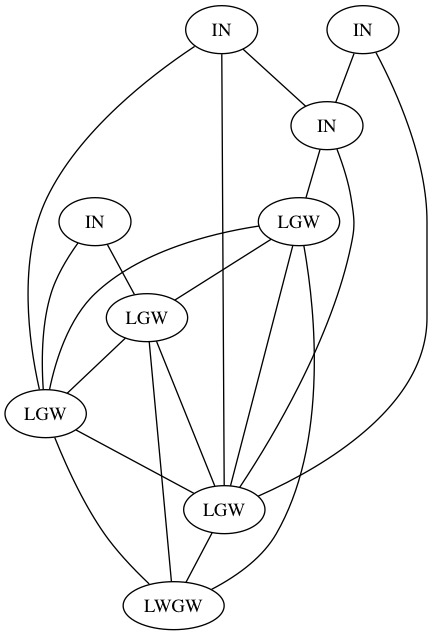
\includegraphics[scale=0.45]{LoRaGraph.jpg} 
\caption{Exemple de Graphe de sortie du script }
\end{figure}
Le code de génération de graphe aléatoire est mis à disposition dans son intégralité en Annexes.
\section{Représentation des échanges radio}
Dans cette version purement algorithmique sur Omnet++, la radio est definit par sa porté qui est donc la possibilité de communiqué avec un device. Si une arrête existe alors une communication est possible. Afin d'être plus réaliste, les arrêtes on pour attribut une latence, qui est générer aléatoirement au moment de la création du graphe. La radio étant des ondes quand un device envoie un message il l'envoie sur tous les liens qui lui sont attribué.

\begin{figure}[!ht]
\centering
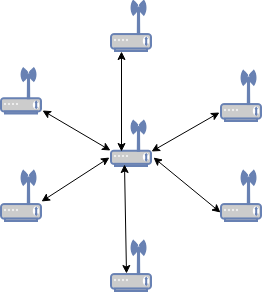
\includegraphics[scale=0.9]{ex_radio.png} 
\caption{Exemple de communication radio}
\end{figure}


\newpage
\section{Exemples de simulations graphiques}
Afin de simplifié, les messages contiennent le nom du message et possedent un code couleur propre et unique. Une \textit{LoRa} Gateway possède une couleur propre à son groupe ( elle même et les Isolated nodes associés), les INs ont aussi cette couleur.
\subsection{Simulation sur une chaine}
\begin{figure}[!ht]
\centering
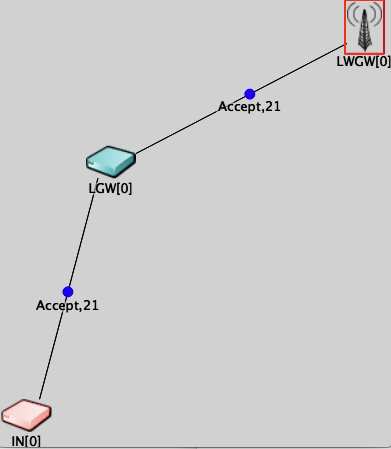
\includegraphics[scale=0.6]{chaine.png} 
\caption{Exemple de chaine}
\end{figure}
Ceci est une image sortie de la simulation graphique, la première réalisé, un exemple typique de chaine avec seulement un élement de chaque composant. C'est le premier exemple de test réalisé. Ce fut aussi le terrain de devellopement pour affiner le comportement individuel et verifier le fonctionnement correct de chaque composant. Cette simulation ci seras l'exemple typique du première algorithme.
\newpage
\subsection{Simulation avec 3 IN sur une LGW}
\begin{figure}[!ht]
\centering
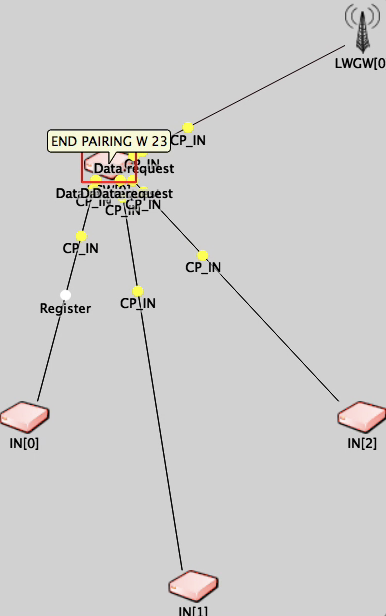
\includegraphics[scale=0.6]{3IN.png} 
\caption{Exemple avec 3 Isolated Nodes}
\end{figure}
Ceci est le deuxième exemple de simulation pour gérer l'enregistrement multiple.Ici nous avons donc toujours une  \textit{LoRaWAN} gateway qui est connecté a une \textit{LoRa} Gateway qui doit gérer trois Isolated Node Cette simulation ci seras l'exemple typique du deuxième algorithme.
\newpage
\subsection{Simulation à plus grande echelle }
\begin{figure}[!ht]
\centering
\includegraphics[scale=0.45]{fat.png} 
\caption{Exemple à grande echelle}
\end{figure}
Ceci est le troisème exemple de simulation pour gérer l'enregistrement multiple ainsi que l'unicité d'un enregistrement sur une Gateway \textit{LoRa} d'un device.Ici nous avons donc toujours une  \textit{LoRaWAN} gateway qui est connecté a quatre \textit{LoRa} Gateway qui doit gérer X Isolated Node Cette simulation ci seras l'exemple typique du deuxième algorithme. Mais aussi d'un troisème cas de figure possible. Cette exemple est surtout présent pour montrer et pousser la simulation à être plus proche de la réalité.
L'exemple présenté ci-contre fait aussi transparaitre les exemples ou les communications sont difficiles. Un noeud peut pendant un certain temps ne faire que envoyer des messages \textbf{Discover} très longtemps. Pour plusieurs raisons, notamment celle-ci : 
\begin{itemize}
\item Problème de latence sur le reseaux de communication. 
\item Problème de bruit radio (Plusieurs emissions sont réalisé en même temps de la part de plusieurs device, que ce soit sur le device de recepetion ou d'émission provocant la corrupition des messages)
\item Problème de phase réception, en effet des slots sont prévue ainsi que deux fenêtre de réception dans la specification \textit{LoRa}. Il se peut que deux device pas encore synchroniser est du mal à l'être .
\end{itemize}

\subsection{Générations des graphes}
Un ensemble de 100 graphes contenant 1000 noeuds on été simulé en respectant cette configuration. 
\begin{itemize}
\item  Variation du nombre de nœuds isolés par passerelle entre 1 et 4.
\item  Variation du nombre de passerelle maximum par puits entre 1 et 4.
\item  Variation du nombre de données à récupérer par jour entre 1 et 24 messages.
\item  Variation sur la méthode de réassemblage des données collectées par les nœuds isolés (ie, envoyé au puits à chaque réception (méthode NA) ou réassemblé après fusion de tous les messages (méthode A))
\item  Variation de la vitesse de chaque lien entre deux nœuds.
\end{itemize}
Ce qui nous fait un total de 12800 graphes à créer. Pour réaliser cette création, nous avons écrit un algorithme basé sur la probabilité d'existence d'un lien entre deux nœuds. C'est-à-dire qu'au début nous créons le premier puits(LWGW). À celui-là regarde son degré (lequel est zéro au début) de la passerelle accrochée à lui. On tire une probabilité et si elle est supérieure à celle établie en entrée de l'algorithme on ajoute une passerelle(LGW) et le lien entre le puits et celui-ci. Nous faisons de même avec les nœuds isolés.
Pour résumer, nous avions:
cent graphiques avec un maximum d'un nœud isolé par passerelle et un maximum d'une passerelle par puits. Cette configuration sera abrégée 1 (IN) -1 (GW) $ \ rightarrow $ 1-1.

Nous avons donc utilisé l'outil Omnet ++ pour simuler tous ces graphes et chaque cas. Dans ceux-ci nous avons noté pour le noeud isolé le nombre de messages envoyés ainsi que la batterie restante à la fin de la simulation.
Pour la batterie, nous avons supposé qu'il avait 6600 mAh ou 23760000 mAs. L'énergie électrique consommée provient de la documentation LoPy, section WiFi. Nos calculs de prévision sont réalisés comme suit:

L'appareil est considéré pour envoyer X msg (\#msg) par jour (sur 24 heures). Le courant d'une émission est Ce = 107,3 ​​mA. Chaque émission dure Te = 2s.
Le courant en réception est Cr = 37mA. L'heure à la réception est Tr
Le courant de veille est Cv = 0,531 mA. L'appareil est inactif pour Tv = (24 * 3600- \#msg * Te-Tr * Cr)
Le courant consommé sur une journée est donc:
CDay (mA.s) = (\#msg * Ceci * Te + Cr * Tr + Cv * Tv)
\subsection{Résultats}
Voici donc un graphique montrant la différence entre le mode d'agrégation et de non-agrégation au niveau du message.
\begin{figure}[htbp]
\centerline{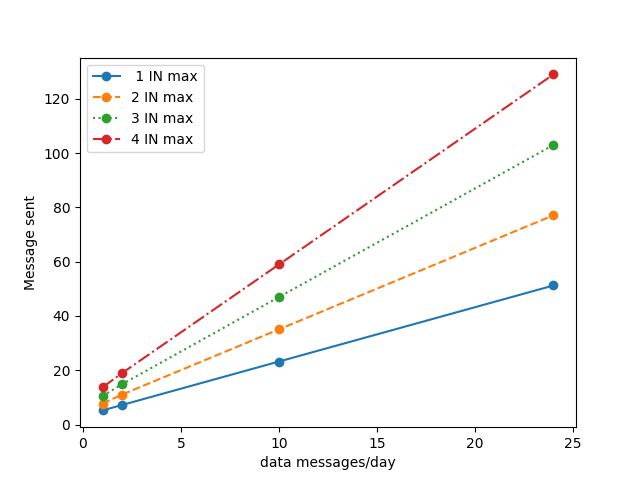
\includegraphics[scale = 0.5]{graphics_resultats/A/A.png}}
\caption{Mode: Agrégation (Concentrateur)}
\label{A}
\end{figure}
On peut remarquer que dans les figures suivantes un aspect linéaire ressort nettement sur la variation du nombre de messages de la part d'une passerelle quel que soit le mode (avec agrégation ou sans agrégation).
\begin{figure}[htbp]
\centerline {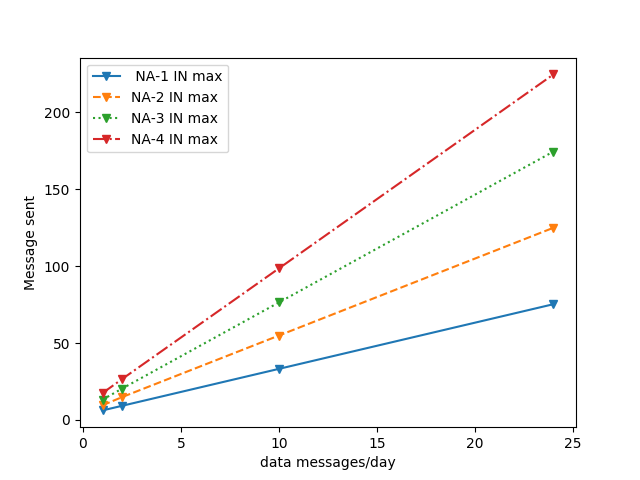
\includegraphics[scale = 0.5]{graphics_resultats/A/NA.png}}
\caption{Mode: Sans d'agrégation (PROXY)}
\label{A}
\end{figure}
Ce que nous pouvons également remarquer est le nombre qui, comme prévu, est plus grand et croît beaucoup plus vite sans le mode d'agrégation (Fig. 4, 5, 6).
Ce qui peut donc être considéré comme suffisamment significatif. En effet, l'ajout des données de la passerelle à celles des noeuds isolés fait que le nombre de messages en mode cluster est le même que si les IN étaient des GW et donc des noeuds connectés.
\begin{figure}[htbp]
\centerline{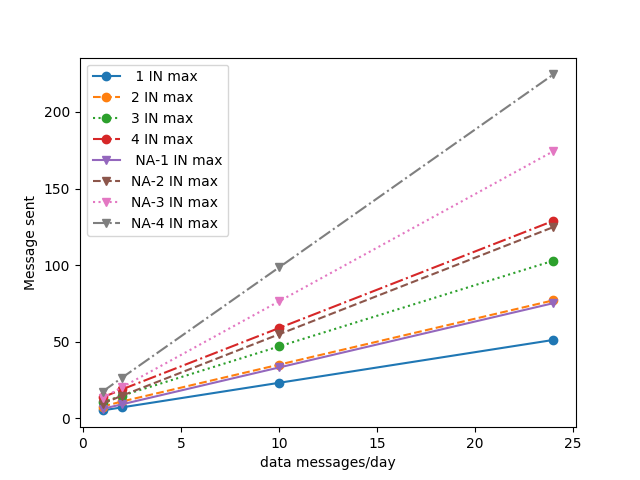
\includegraphics[scale = 0.5]{graphics_resultats/A/AvsNA.png}}
\caption{Mode: Concentrateur vs Proxy}
\label{A}
\end{figure}

L'objectif était de vérifier si l'idée intuitive est correcte: l'architecture avec relais intermédiaire et agrégation renvoie, en nombre de messages et donc de durée de vie du réseau, au modèle sans relais, le modèle ou chaque client parle en direct avec des antennes toujours UP.

Les figures 7 à 10 sont plus complexes. En effet ces graphes représentent par leurs couleurs le nombre de Gateway maximum lié à un puits. Chaque point est un rappel de simulation décrit par le degré maximum de passerelles et de nœuds isolés ainsi que le nombre de messages demandés par le puits par jour. Ici, ces quatre figures sont en mode d'agrégation.

D'abord sur chaque graphique, chaque point est une moyenne du nombre de messages envoyés ou de l'état de la batterie le cas échéant, par un nœud isolé, ou par une passerelle si nécessaire. Pour chaque graphe, le bloc de 4 couleurs est donc l'ensemble des graphes de degré 1 IN. il faut comprendre que les simulations de 0 à 399 sont celles appelées "1-1, 1-2, 1-3, 1-4". de 400 à 799 "2-1, 2-2, 2-3, 2-4" etc.
Nous avons réalisé ces simulations avec comme précédemment dit un nombre de message demandé par les différents puits. En effet nous avons choisi: 1, 2, 10, 24 messages par jour.
\begin{figure}[!ht]
\centerline {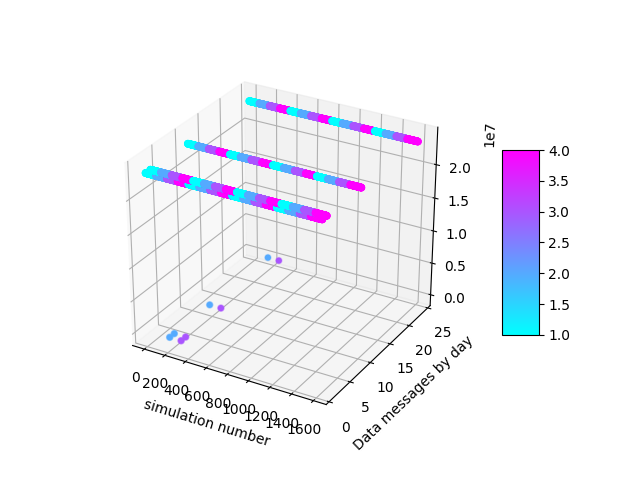
\includegraphics[scale=0.5]{graphics_resultats/bat/Sim_MSG_SEND_data_bat_gw_degree_gw.png}}
\caption {Etat de la batterie sur un jour / message de données requis / jour pour une passerelle}
\label{A}
\end{figure}

\begin{figure}[!ht]
\centerline{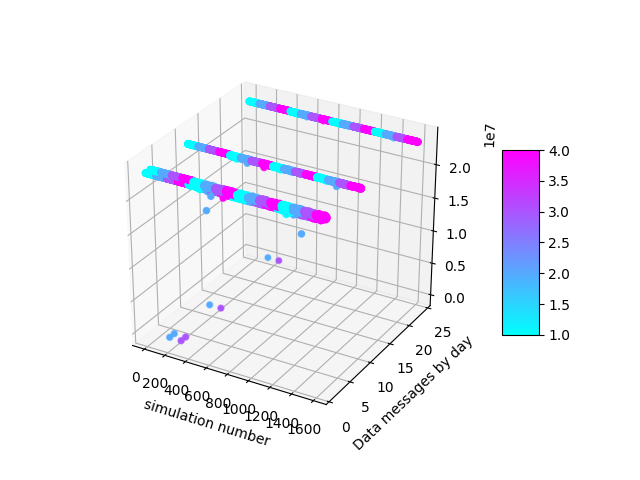
\includegraphics[scale = 0.5]{graphics_resultats/bat/Sim_MSG_SEND_data_bat_in_degree_GW.png}}
\caption{Etat de la batterie sur un jour / message de données requis / jour pour un IN}
\label{A}
\end{figure}


\begin{figure}[!ht]
\centerline {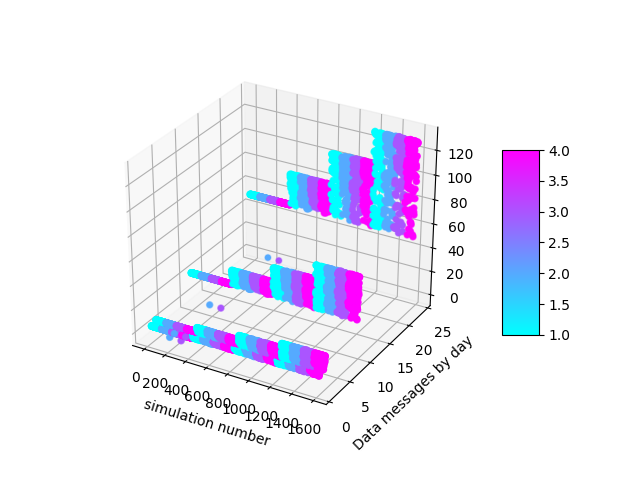
\includegraphics[scale = 0.5]{graphics_resultats/msg/Sim-MSG_GW-MSG_SEND-degree_GW.png}}
\caption {Nombre de messages sur un jour / message de données}
\end{figure}% ok correction ? 
\chapter{Programmation}
%
\chapter{Problème}
\section{Solutions de chiffrement possibles LGW <->IN}
Afin de valider si le n\oe{}ud isolé attaché à une LoRaGateway est bien connu de la part de Spot. Il nous faut récupérer les informations afin de réaliser le mode proxy. C'est à dire, MIC, NwkSkey, AppSkey, DevEui, DevNonce, AppNonce, AppKey NetID. Ces informations sont évidemment soumises à plusieurs degrés de sensibilité. Il a été convié que l'AES 128 bits, est une solution assez satisfaisante. Ce qui assure donc une sécurité de bout en bout en AES-128.

\begin{figure}[!ht]    \centering
   
\includegraphics[scale=0.6]{aes-128.png} 
   \caption{Schéma récapitulatif sur le chiffrement}
   \label{Schéma récapitulatif sur le chiffrement}
\end{figure}
Maintenant il y a un choix important à réaliser, en effet l'AES-128 est du chiffrement symétrique. Il est nécessaire de choisir une clé qui doit être connue des deux partis (Device A et B) . \\
Nous avons donc choisi d'utiliser l'échange de clés Diffie-Hellman, qui est une méthode, publiée en 1976, par laquelle deux agents, nommés par convention Alice et Bob, peuvent se mettre d'accord sur un nombre (qu'ils peuvent utiliser comme clé pour chiffrer la conversation suivante) sans qu'un troisième agent appelé Ève puisse découvrir le nombre, même en ayant écouté tous leurs échanges. \\

Voici un déroulement de base tel que nous le concevons lors de la mise en place sur une LoRaGateway et un Isolated node.\\
La LoRaGateway choisit un nombre premier P et une base G. (P et G premier entre eux ). Dans notre exemple, P=23 et G=3\\
la LoRaGateway choisit un nombre secret a=6\\
Elle envoie à Bob la valeur A = $g^a$ [mod P] = $3^6$ [23] = 16\\
Bob choisit à son tour un nombre secret b=15\\
Bob envoie à la LoRaGateway la valeur B = $G^b$ [mod P] = 3\up{15} [23] = 12\\
la LoRaGateway peut maintenant calculer la clé secrète : $B^a$ [mod P] = $12^6$ [23] = 9\\
Bob fait de même et obtient la même clé que la LoRaGateway : $A^b$ [mod P] = 16\up{15} [23] = 9\\

Pour faire simple, La LoRaGateway peut transmettre toutes les données nécessaire en clair c'est à dire P, G, A  à un n\oe{}ud isolé et cela sans aucun soucis. Puisque pour déduire la clé résultante il faut résoudre l'impossibilité (calculatoire) de déduire des seules informations $g^a$, $g^b$, G et P, la valeur de G\up{ab} .
il faut toutefois parler du problème de l'attaque classique du Man in the middle. La parade classique à cette attaque consiste à signer les échanges de valeurs à l'aide d'une paire de clés asymétriques certifiées par une tierce partie fiable, ou dont les moitiés publiques ont été échangées auparavant par les deux participants.

\section{Problème final }
Lors d'un test rapide, la plupart des services qui utilisent l'algorithme de Diffie-Hellman, est gérée par la bibliothèque libre OpenSSL. La force de cet algorithme réside aussi dans les principes mathématiques qu'entourent les nombres premiers, tout comme pour l'algorithme RSA, plus le nombre premier choisi est grand plus la sécurité en est renforcée. Or plus un nombre est grand.. plus il faut s'attendre à gérer des opérations mathématiques très lourdes, en plus de la recherche initiale du nombre premier. Ce qui rappelons le, peut être assez long compte tenu de la puissance de calcul dont dispose un capteur. Ceci n'est que le problème au niveau de la recherche de P. En effet on parle d'une élévation à la puissance (dans la suite du calcul) d'un nombre déjà extrêmement grand, en effet il faut s'attendre à exploser la capacité maximale que peut engranger un nombre en informatique c'est à dire : 18 446 744 073 709 551 615 == 2\up{64}-1 . Pour résoudre ce souci OpenSSL utilise la bibliothèque BIGNUM en C . Qui comme la lib OpenSSL n'est pas disponible sur les capteurs sur lesquels nous développons. 
\section{Conclusion sur le chiffrement}
Il y a plusieurs piste à envisager, celle dont-on parle dans ce document part du principe que nous n'avons aucune autre entrée sécurisée donnée par la LoRaWAN Gateway lors d'un join. La solution à ce problème est probablement du côté des fonctions de type courbes elliptiques comme celles de Diffie-Hellmann . Pour faire simple une solution basée sur les courbes elliptiques serait non implémentable \textbf{sans secure element} . Il est donc nécessaire d'envisager une autre piste. 

% ok correction ? 
\chapter{Bilan}

\begin{center} 
\end{center}

%Rappel des résultats

%Conclusion/Perspectives


 


\newpage

%Ne pas numéroter cette partie
\part*{Annexes}
%Rajouter la ligne "Annexes" dans le sommaire
\addcontentsline{toc}{part}{Annexes}

%
%
%%changer le format des sections, subsections pour apparaittre sans le num de chapitre
%\makeatletter
%\renewcommand{\thesection}{\@arabic\c@section}
%\makeatother
%
%%recommencer la numérotation des section à "1"
%
%%\addcontentsline{toc}{subsection}{Organisation tests CPU}
%\begin{figure}
%\centering
%\includegraphics[angle=90,scale=0.35]{images/grapheCPU.png}
%\caption{Graphe d'organisation des tests du CPU}
%\end{figure}
%
%
%%\addcontentsline{toc}{subsection}{Organisation tests HDD}
%\begin{figure}
%\centering
%\includegraphics[angle=90,scale=0.45]{images/grapheHDD.png}
%\caption{Graphe d'organisation des tests HDD}
%\end{figure}
%
%
%
%
%%\addcontentsline{toc}{subsection}{Organisation tests network}
%\begin{figure}
%\centering
%\includegraphics[angle=90,scale=0.40]{images/grapheNT.png}
%\caption{Graphe d'organisation des tests sur le network}
%\end{figure}
%
%%\addcontentsline{toc}{subsection}{Organisation du stage}
%\begin{figure}
%\centering
%\includegraphics[angle=90,scale=0.5]{images/graphe.png}
%\caption{Graphe d'organisation du stage}
%\end{figure}
%%\addcontentsline{toc}{subsection}{Organisation sonde personnelle}
%\begin{figure}
%\centering
%\includegraphics[scale=1]{images/fat.png}
%\caption{Graphe d'organisation de type Fat tree}
%\end{figure}



\input{./annexe2.tex}

\newpage
\begin{thebibliography}{9}

   \bibitem{Docker}
          Documentation Docker
          \url{https://docs.docker.com/}.

\end{thebibliography}


\end{document}